In diesen Kapitel wird die Problemstellung der Reparatur und die im Paper als
state-of-the-art bekannten Reparaturmethoden vorgestellt. Die Reparatur mit
der Anomalienerkennung wird im zweiten Kapitel entscheidend, da die im Paper als
neue Methodik vorgestelltes IMR iterativ auf ARX aufbaut.  Die Stellvertreter
der anderen Methoden werden zusätzlich bei der Evaluierung von IMR für den
Vergleich herangezogen.

\subsection{Problemstellung der Reparatur}

Es sei $x = x[1],\dots,x[n]$ eine Zeitreihe, die aus einer Messung erhoben
wurde und tendenziell unkorrekte Werte enthalten kann. Kurz wird ein
Datenpunkt $x[i]$ mit $x_i$ für jeden Zeitpunkt $i \in
\{1,2,\dots,n\}$ bezeichnet. Zudem sei $x^{\text{truth}}$ dieselbe Zeitreihe
mit unvollständigen, aber dafür absolut korrekten Werten; kurz markierte Werte.
\[
    x^{\text{truth}}_i = \left\{
\begin{array}{ll}
    x^{\text{truth}}_i = w_i&, \text{falls ein korrekter Datenpunkt }w_i
    \text{ für den Zeitpunkt }\\
&~ i \text{ bekannt ist.}\\
    \text{\_\_}&, \text{ansonsten}
\end{array}
 \right.
\]
Neben diesen beiden Zeitreihen sei $x^{\text{truth*}}$ die vollständig bekannte
und absolut korrekte Zeitreihe. Gesucht ist ein Verfahren, das für eine beliebige
Zeitreihe $x$ und ein zugehöriges $x^{\text{truth}}$ eine reparierte Zeitreihe
$y$ ohne der Kenntnis von $x^{\text{truth*}}$ ermittelt, sodass die Abweichung von y
zu $x^{\text{truth*}}$ minimal ausfällt. Jeder bekannte Wert von
$x^{\text{truth}}$ ist dann in $y$ enthalten. Lediglich Werte in y, die in
$x^{\text{truth}}$ unbekannt bzw.\ auf \_\_ gesetzt sind, sind die reparierten
Werte von $x$.
\\
\\
Eine Abweichung ist hierbei minimal, wenn der RMS-Fehler $\Delta$ minimal ist:
\[
    \Delta\left(x^{\text{truth*}}, y\right) = \sqrt{\frac{1}{n} \sum_{i=1}^n \left( x^{\text{truth*}}_i - y_i \right)^2}
\]
Im Gegensatz zu der euklidischen Distanz als Abweichungsfunktion werden bei RMS temporär stärkere Abweichungen deutlich stärker bestraft.
~\\
\\
\textbf{Beispiel 1}. Es seien folgende Zeitreihen $x$, $x^{\text{truth}}$, $x^{\text{truth*}}$ und eine Reparatur $y$ gegeben:
\begin{itemize}
    \item $x =                 \{6, 10, 9.6, 8.3, 7.7, 5.4, 5.6, 5.9, 6.3, 6.8, 7.5, 8.5\}$
    \item $x^{\text{truth}} =  \{6, 5.6, 5.4,  \_\_, \_\_,5.4, \_\_,\_\_,\_\_,\_\_,\_\_,8.5\}$
    \item $x^{\text{truth*}} =  \{6, 5.6, 5.4,  5.2, 5.3, 5.4, 5.6, 5.9, 6.3, 6.8, 7.5, 8.5\}$
    \item $y =  \{6, 5.6, 5.4,  5.2, 5.4, 5.4, 5.6, 5.9, 6.3, 6.8, 7.5, 8.5\}$
\end{itemize}
\begin{figure}
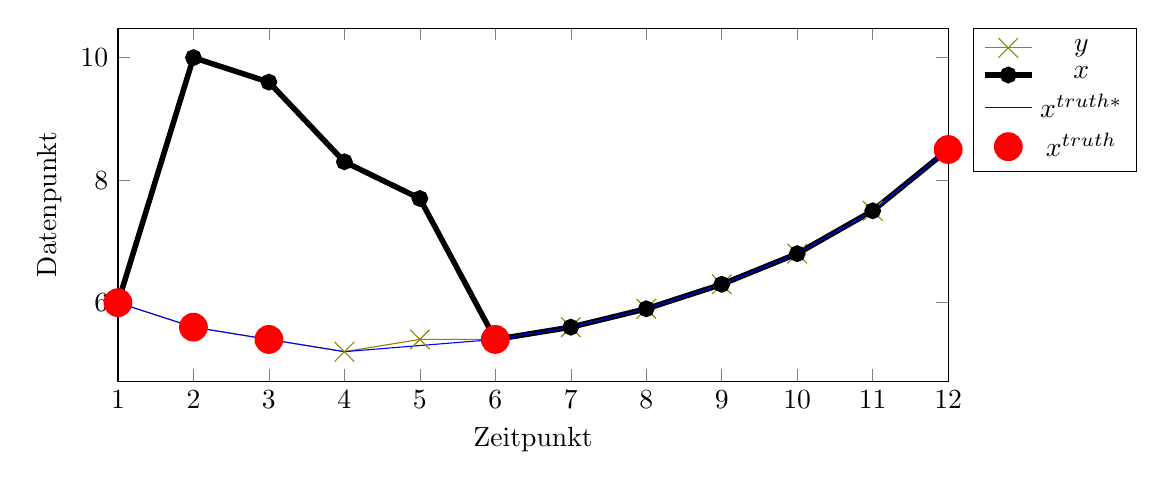
\begin{tikzpicture}
\begin{axis}[width=\textwidth,
    height=.5\textwidth,
xlabel=Zeitpunkt,
ylabel=Datenpunkt,
legend pos=outer north east,
xmin=1,
xmax=12
]
\addplot[olive,mark size=5.0pt, mark=x] table{
Zeitpunkt Wert 
1 6
2 5.6
3 5.4
4 5.2
5 5.4
6 5.4
7 5.6
8 5.9
9 6.3
10 6.8
11 7.5
12 8.5
};
\addlegendentry{$y$}
\addplot[black, line width=2.0pt, mark size=2.0pt, mark=*]  table{
Zeitpunkt Wert 
1 6
2 10
3 9.6
4 8.3
5 7.7
6 5.4
7 5.6
8 5.9
9 6.3
10 6.8
11 7.5
12 8.5
};
 \addlegendentry{$x$}
    \addplot[blue,mark size=5.0pt] table{
Zeitpunkt Wert 
1 6
2 5.6
3 5.4
4 5.2
5 5.3
6 5.4
7 5.6
8 5.9
9 6.3
10 6.8
11 7.5
12 8.5
};
\addlegendentry{$x^{\text{truth*}}$}
\addplot[only marks, red, mark size=5.0pt] table{
Zeitpunkt Wert 
1 6
2 5.6
3 5.4
6 5.4
12 8.5
};
\addlegendentry{$x^{\text{truth}}$}
% if you have the file, you can do
% \addplot table {datafile.csv};
\end{axis}
\end{tikzpicture}
    \caption{Beispiel 1.}\label{fig:1}
\end{figure}
~\\
In der Abb.\ \ref{fig:1} sind die Zeitreihen eingetragen. Es lässt sich
erkennen, dass Messfehler bei den Zeitpunkten 2 bis 5 durch eine nach oben
angeordnete Verschiebung der Werte auftreten. Die Messungen bei den anderen
Zeitpunkten sind hingegen korrekt.  Es lassen sich zwei Vorteile durch das
Hinzunehmen von markierten Werten $x^{\text{truth}}$ erkennen.  Einerseits
können die Werte direkt in die Reparatur $y$ einfliessen, andererseits kann
durch die Ermittelung der Abweichungen zu den Messungen geschlussfolgert
werden, dass die umliegenden Zeitpunkte einen ähnlichen oder keinen Fehler
aufweisen.  Letzteres wird ebenfalls von ARX und die darauf aufbauende IMR
ausgenutzt (siehe Kapitel \ref{sec:anomalienerkennung} und \ref{sec:IMR}). In
der Darstellung stimmen die Messungen bei 6 und 12 mit den markierten Werten
überein, sodass die Annahme gemacht werden kann, dass die Messungen 7 bis 11
mit hoher Wahrscheinlichkeit ebenfalls korrekt sind.  Aufgrund von den zu
beobachtenden absteigend größeren Fehler von Zeitpunkt 2 bis 3 lässt sich die
Vermutung aufstellen, dass die Zeitpunkte 4 und 5 ebenfalls diesen Abwärtstrend
eines Fehlers unterliegen. Die Reparatur $y$, welcher mithilfe des Verfahrens IMR
bestimmt wurde, setzt diese Vermutungen um.  In der Darstellung kann lediglich
ein geringer Fehler der Reparatur $y$ bei Zeitpunkt 5 festgestellt werden. Der
RMS-Fehler $\Delta$ liegt hier bei $0.03$.   

\subsection{State-of-the-art Repariermethoden}
Die Qualität der Daten spielt eine wichtige Rolle für die Korrektheit
eines statistischen Modells. Um besser vorhersagen zu können, sollte ein Modell
von saubere Daten lernen. Deswegen müssen immer Datensätze auf Qualität geprüft
werden und entsprechend bereinigt werden. Durch die hohe Menge an Daten, die
man heutzutage hat, ist die automatische Erkennung und Reparatur von
fehlerhafte Datensätze von große Bedeutung.

\subsubsection{Reparatur mit Anomalienerkennung}\label{sec:anomalienerkennung}
Unter Anomalienerkennung versteht man die Suche nach unerwartete Daten in einem
Datensatz. Diese unerwartete Werte können sowohl stark als auch schwach von dem
erwarteten Wert abweichen. Die unsaubere Daten werden erst nach bestimmten
Kriterien als Anomalien erkannt. Oft wird ein Wert als Anomalie gekennzeichnet,
falls der betrachtete Wert $x_t$ sich vom erwartetem $x_t'$ um eine Konstant
$\tau$ unterscheidet. Für die Zeitreihenvorhersage gib es zwei gut etablierte
Modelle (AR und ARX), die den erwarteten Wert $x_t'$ für den Zeitpunkt $t$ vorhersagen
können. Außerdem sind beide dieser Methoden modifizierbar um mögliche Anomalien
zu reparieren.
\begin{itemize}
  \item \textbf{Autoregressives Modell (AR)}\\
  Dieses Modell ist nichts anderes als ein Art Lineare Regression. Die Ausgabe $x_t'$
  ist linear abhängig von den vergangenen Werten $x_{t-i}$ für $i\in[1,..,p]$ und
  eine Zufallsvariable $\epsilon_t$. Diese Zufallsvariable wird normalerweise
  als Weißrausch bezeichnet ($\epsilon_t \sim \mathcal{N}(0,\,\sigma^{2}) $).
  Das Modell $AR(p)$ ist definiert durch:
  \[
  x_t'=\sum_{i=1}^{p}\phi_ix_{t-i}+\epsilon_t
  \] 
  \begin{figure}[h]
      \centering
      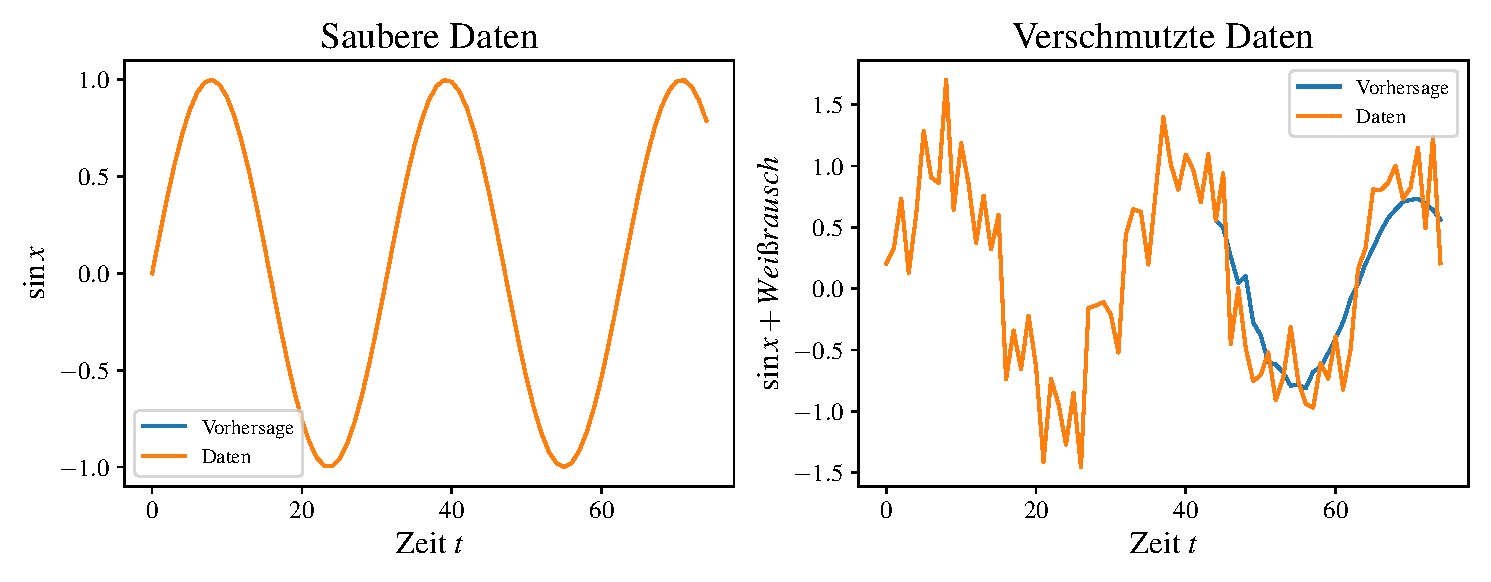
\includegraphics[width=\textwidth,keepaspectratio]{../plots/ar_sauber_verschmutze_daten.pdf}
      \caption{Beispiel eines AR(30) Modells an eine Sinuskurve(Links) und eine
      Sinuskurve mit Rausch(Rechts)}
      \label{fig:ar}
  \end{figure}
  Die Parameter $\phi_i$ können analytisch mit der Hilfe der Methode der
  kleinsten Quadrate errechnet werden, siehe Abbildung \ref{fig:ar}. Die Lösung den Parametern $\phi$ ist
  durch die Gleichung
  \[
    \phi = (X^TX)^{-1}X^TY
  \]
  gegeben, wo $Y$ ein Vektor der Länge $|n-p|$ ist 
  \[
    Y = 
    \begin{bmatrix}
    x_{p+1}\\
    x_{p+2}\\
    \vdots\\
    x_{n-1}\\
    x_{n}
    \end{bmatrix}
  \]
  , der eingangs Vektor $X$ mit Zeit verzögerte Werte 
  \[
    X = 
    \begin{bmatrix}
    x_{p}&x_{p-1}&\hdots&x_{1}\\
    x_{p+1}&x_{p}&\hdots&x_{2}\\
    \vdots&\vdots&\ddots&\vdots\\
    x_{n-2}&x_{n-3}&\hdots&x_{p+1}\\
    x_{n-1}&x_{n-2}&\hdots&x_{n-p}
    \end{bmatrix}
  \]
  und \[
  \phi=
    \begin{bmatrix}
    \phi_{1}\\
    \phi_{2}\\
    \vdots\\
    \phi_{p-1}\\
    \phi_{p}
    \end{bmatrix}
  \]
  Um eine Reparation der Werte durchzuführen, werden zuerst alle $x_t$ durch
  $y_t$ getauscht für alle markierte $x_t$. Sei $x^{truth}$ eine Liste von den
  markierten Werte in $x$, dann kann man diese Werte für das lernen der
  Parameter $\phi$ benutzen um eine genauere Vorhersage der Werte ohne
  Markierung $x\setminus x^{truth}$ vorzunehmen. Um mit AR eine Reparatur
  vornehmen zu können, vergleicht man den Abstand einer nicht markierten Wert
  $x_t$ zu $x_t'$ mit einem Schwellenwert $\tau$. Falls diese den Schwellenwert
  überschreitet, repariert man den gegebenen Wert mit der Vorhersage $x_t'$.
  Anderseits lässt man den alten Wert $x_t$ stehen. Also,
  \[
    y_t= 
    \begin{cases}
    x_t'& \text{falls} \,|x_t'-x_t|>\tau\\
    x_r              & \text{sonst}
    \end{cases}
  \]
    \item \textbf{Autoregressives exogenes Modell (ARX)}\\
    Ebenso, wie beim AR(p), kann man das lineare Modell ARX benutzen um eine
    Reparatur der Daten durchzuführen. Wie schon erwähnt, AR(p) nimm im
    Betracht die vergangene Werte $x_i$ für $i<t$ als Parameter um die nächste
    Wert $x_t$ zu bestimmen. Im Gegensatz zu AR(p), ARX(p) nutz die information
    von $y_i$ für $i<t$ aus. Sei $y$ die liste mit den reparierte bzw. als
    Wahrheit markierte Werte von $x$, dann ist ARX(p) (Abildung \ref{fig:arx})
    definiert als, 
    \[
      y_t'=\sum_{i=1}^{p}\phi_i(y_{t-i}-x_{t-i})+\epsilon_t\quad.
    \]
    \begin{figure}[h]
      \centering
      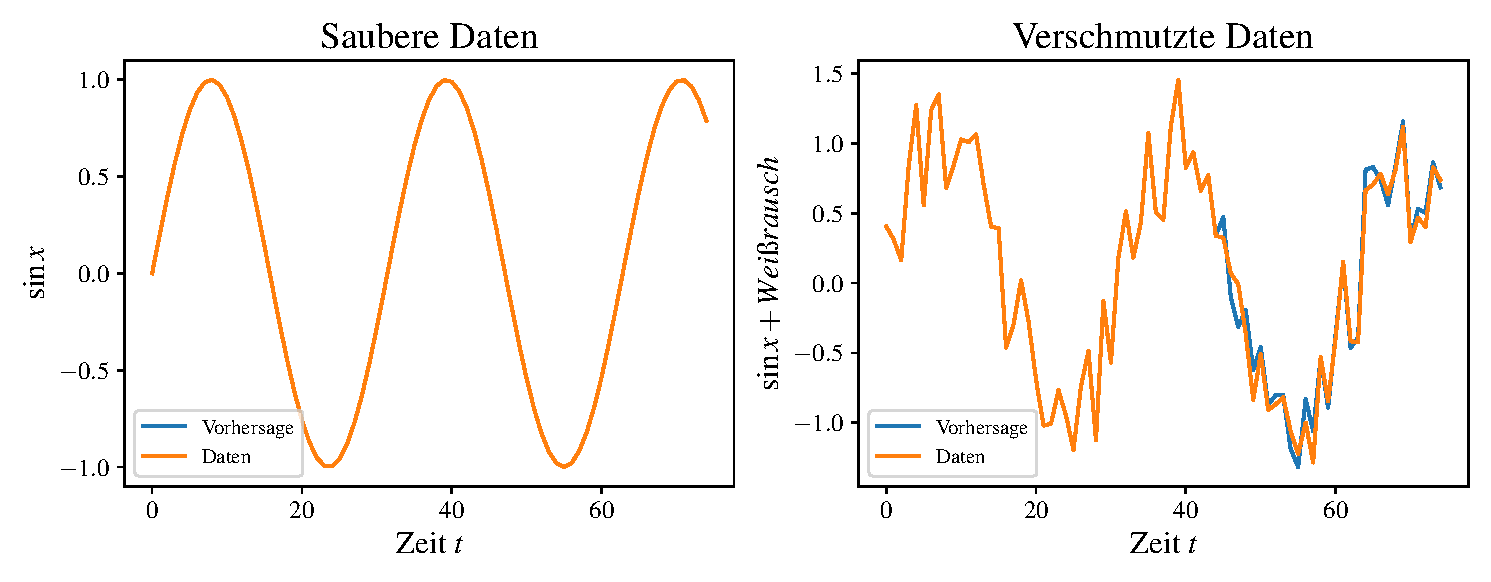
\includegraphics[width=\textwidth,keepaspectratio]{../plots/arx_sauber_verschmutze_daten.pdf}
      \caption{Beispiel eines AR(30) Modells an eine Sinuskurve(Links) und eine
      Sinuskurve mit Rausch(Rechts)}
      \label{fig:arx}
    \end{figure}
    Die Reparatur der Reihe funktioniert dann genauso wie beim AR Modell.
\end{itemize}
\subsubsection{Bedingungsbasierte Reparatur}
Es gibt auch Daten, die vom erwartete Werte abweichen aber die abweichung is
nicht so startk. 
Es werden nicht alle daten benutz
Hinterienander fehlerhafte Daten können falsch interretiert werden
Die reparierte Reihe y

\begin{itemize}
  \item Was ist Bedingungsbasierte Reparatur (siehe 7.3)
  \item SCREEN (vgl.\ referenzierte Papers) 
  nimm in betrach nur ein punkt
\end{itemize}
\subsubsection{Glättungsbasierte Reparatur}
Gleitender Mittelwert
\begin{figure}[h]
      \centering
      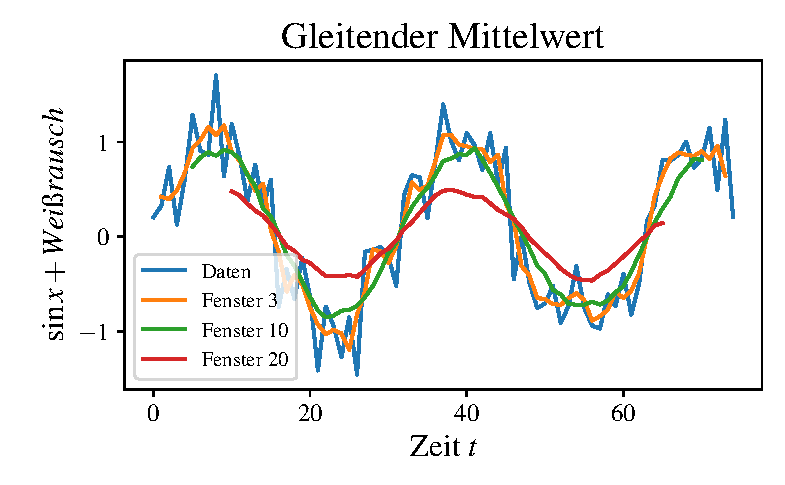
\includegraphics[width=\textwidth,keepaspectratio]{../plots/Gleitender_Mittelwert.pdf}
      \caption{Beispiel mehrere Gleitender Mittelwert der 
      Verschmutze Daten mit Fenster Große 3, 10 und 20}
      \label{fig:rolling}
\end{figure}
\begin{itemize}
  \item Was ist Glättungsbasierte Reparatur (siehe 7.2)
  \item EWMA (vgl.\ referenzierte Papers) 
\end{itemize}

